\chapter{Heavy Ion Collisions: A Primer} % Main chapter title
\label{hicollisions}
%----------------------------------------------------------------------------------------
\section{Measurable Quantities}
Due to the complexity inherent in colliding large nuclei containing a large number of nucleons (for instance 197 nucleons in Au) there is a multitude of metrics we can use to quantify the collision and the evolution of what happens after. For clarification, when talking about high energy physics analyses we refer to all data gathered from a single collision of two nucleons as an \textit{event}. The location where the collision takes place is called the \textit{event vertex} or often in collaboration literature since the z-axis is along the beam axis, the \textit{z vertex}. The high luminosity of heavy ion collisions (437 $nb^{-1}$ in 9 weeks for the data used in this analysis: Run 8 d+Au), produces a plethora of particles. As these particles travel from the event vertex through the various layers of detectors under the influence of the PHENIX magnetic field it leaves its own signature on each detector it passes through. These signatures for each given particle can be matched to form a trajectory from the event vertex through PHENIX. The set of data corresponding to location, kinematic, and detector specific variables (i.e. charge deposited, clusters fired, Cherenkov photons, etc) is called a \textit{track}. The determination of these variables is the topic of this chapter.

\section{Event Characterization}
When describing a heavy ion collision it is useful to introduce quantities that describe the initial conditions of the interacting nucleons. The set of variables that correspond to these conditions are called the \textit{event} or \textit{global} variables. They are used to accurately locate where the event took place inside the detector and the geometric configuration of the nuclei at the time of collision. Since we are accelerating the ions to ultra relativistic speeds, by Heisenberg uncertainty we have very little idea before the collision what event parameters such as centrality and event plane will be. In practice, we use the remnants of the collisions to determine these event parameters and since the particles that are largely unperturbed by the collision are the ones that do not interact but rather continue down the beam pipe, these event variables reconstructed mostly by the extremely forward detectors: the \textit{Beam-Beam Counters} (BBC) and the \textit{Zero Degree Calorimeters}. 

\subsection{Centrality}
One such variable is \textit{centrality} and is used to describe how "head-on" two ions collide, that is, do they collide with complete cross sectional overlap or do they just barely glance each other. It is useful to quantify this overlap with a quantity called the \textit{impact parameter}, \textbf{b}. We define this impact parameter by measuring the distance between ion centers as depicted on the left-hand side of figure \ref{fig:cernfireball}. Note that the ions in this illustration appear squished in the x axis due to Lorentz contraction. Therefore, small impact parameters correspond to large ion-ion overlap in the collision and large impact parameters refer to glancing collisions. In heavy ion physics we call collisions with small impact parameters \textit{central collisions} and those with large impact parameters \textit{peripheral collisions}. Experimentally it is impossible to measure the distance between the two ion centers. In practice, centrality can also be quantified by the number of \textit{participants}, or the number of nucleons that collide/interact with each other, versus the number of \textit{spectators}, or the number of nucleons that do not collide. Since we know the number of total nucleons in each ion we can determine the number of participants by counting the number of spectators and subtracting them from the total number of nucleons. Colliding nucleons will produce particles in all directions however spectating nucleons will continue to travel down the beam pipe. We therefore can count the number of spectators by placing detectors at very high rapidity.

\begin{figure}[htbp!]
  \centering
    \begin{subfigure}[p]{1\textwidth}
    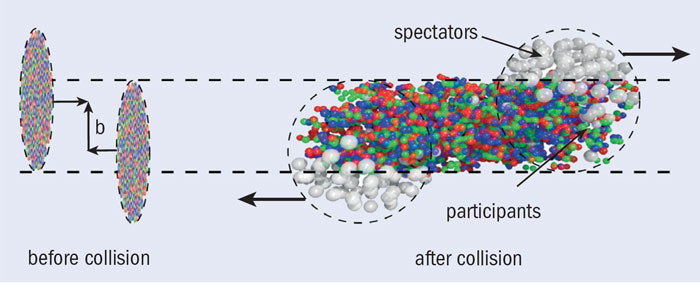
\includegraphics[width=1\textwidth]{Figures/spectatorsvsparticipants.jpg}
    \caption[Diagram showing impact parameter versus $N_spectators$ and $N_participants$]{Diagram showing impact parameter versus $N_spectators$ and $N_participants$\citep{cernhifireball}}
    \label{fig:cernfireball}
    \end{subfigure}
    \begin{subfigure}[p]{1\textwidth}
    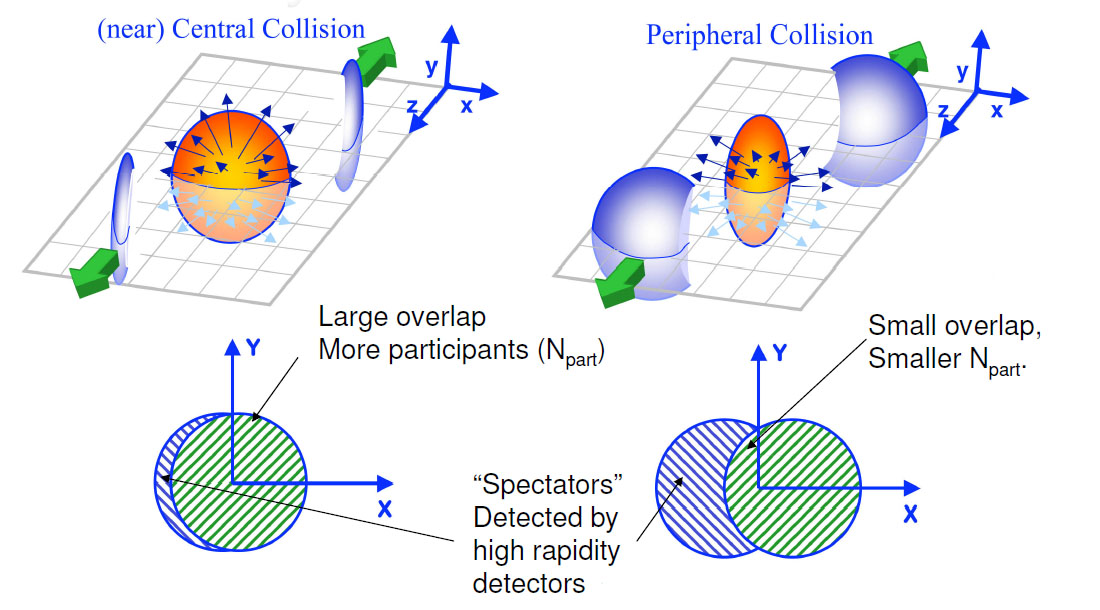
\includegraphics[width=1\textwidth]{Figures/centralvsperipheral.jpg}
	\caption[Central vs Peripheral collisions, geometry of initial conditions]{Central vs Peripheral collisions, geometry of initial conditions.}
    \end{subfigure}
    \rule{35em}{0.5pt}
  \caption[Central versus peripheral ion collisions, BBC vs ZDC determination of]{Central versus peripheral ion collisions, BBC vs ZDC determination of}
  \label{fig:centralvsperipheral}
\end{figure}

Extending the terminology from impact parameters, we then define a collision with a large number of participants to be a \textit{central} collision and a collision with a small number of participants: a \textit{peripheral} collision. These are quantified in percents, 0$\%$ being most central collisions i.e. highest number of participants, $b=0$, two colliding ions overlap completely, and 100$\%$: ions completely miss each other, i.e. there are no participants, $b > R_{nucleus}$. Since ions are spherical in shape, centrality can be used as a way of describing the geometry of the collision region, central collisions have a more circular shape whereas peripheral collisions have a more almond-like shape.



\subsection{Event Vertex and Timing}
The event vertex is the location along the beam axis where the collision happened relative to the equidistant point between the two beam beam counters. That is, an event vertex value of 0 would be exactly in the center of the PHENIX detector, at equal distance from both BBCs. When a collision happens, the non colliding nucleons (spectators) continue to travel through the interaction region and are detected on the other side by the two BBCs. The time at which each cluster of spectators hits an individual BBC is measured. These two times, $T_1$ and $T_2$ respectively, can be used to calculate both the event vertex ($z_{vtx}$) and the initial time the collision takes place ($T_0$) as follows\citep{Mitchell:2002wu}:

\begin{equation}
 z_{vtx} = \frac{T_1 - T_2}{2c} \qquad\text{and}\qquad T_0 = \frac{T_1 + T_2}{2}
\end{equation}

This initial time is used to start the stopwatch of the event and is used in conjunction with other detectors to to find the time a produced particle takes to travel from the vertex to a detector.

\begin{figure}[htbp!]
  \centering
    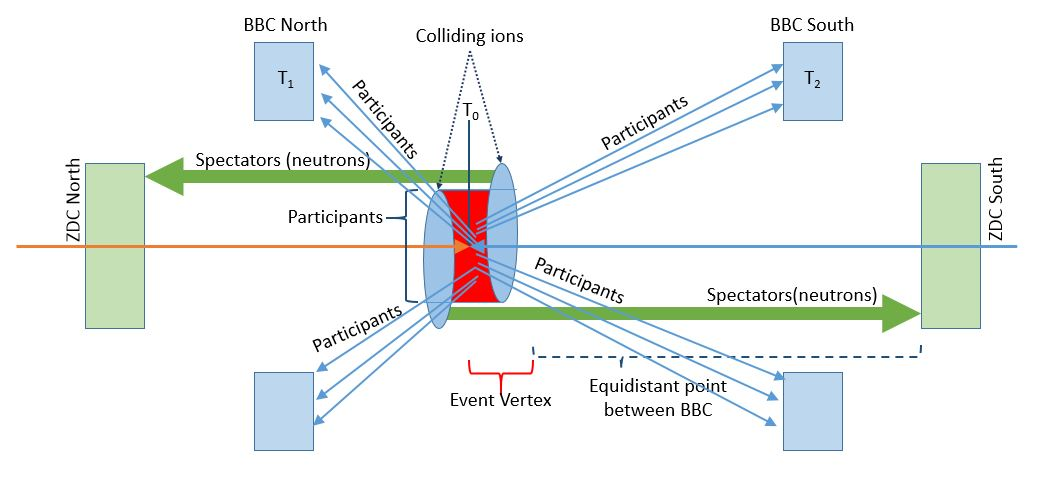
\includegraphics[width=1\textwidth]{Figures/BBCevtchar.JPG}
    \rule{35em}{0.5pt}
  \caption[Diagram of BBC event characterization]{Diagram of BBC event characterization}
  \label{fig:bbcvtx}
\end{figure}


\begin{figure}[htbp!]
  \centering
    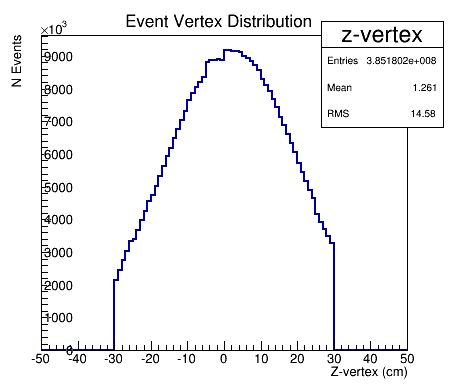
\includegraphics[width=0.5\textwidth]{evtQA/zvtxdist.JPG}
    \rule{35em}{0.5pt}
  \caption[Event Vertex Distribution]{Event vertex distribution, there is an applied cut for all events to be $|z_{vtx}| \geq 30$ cm.}
  \label{fig:vtxdist}
\end{figure}

\section{Track Reconstruction}
\label{trkrecosect}
\subsection{Variables for Track Selection}
After the collision, particles fly outward from the vertex under the various mechanisms that take place within the formation and evolution of the QGP. Due to the high multiplicity of tracks resulting from a heavy ion collision and the various complexities that arise when using a multifaceted complicated detector system to reconstruct track trajectories, it is important to come up with a metric by which to measure the quality of the tracks in order to discern which tracks are able to be reconstructed cleanly versus those which, for whatever anomalous reasons, would not be advantageous to analyze.
\subsubsection{Track Matching: DC and PC1}
The process of determining the track trajectory through the PHENIX detector is called \textit{track matching} and it utilizes the various layers of the Drift Chamber and Pad Chambers in concert to determine track momentum due to the varying curvature of tracks of different momenta traveling through a magnetic field. Tracks are reconstructed in the DC and PC1 using an algorithm called a \textit{combinatorial Hough Transform} (CHT) which works very well for particles whos $p_T$ is $>$200 MeV/c \citep{Mitchell:2002wu}. CHT is a methodical continuation of a \textit{Hough Transform} which is a reconstruction algorithm used on a set of points that we know were created by single linear tracks in order to fit them with likely linear track candidates\citep{OHLSSON199277}. We use a parameter called track \textit{quality} in order to quantify our confidence that a CHT reconstructed track is a likely fit and it is a function of how well a reconstruction fits hits in the different tracking detector layers (X1, X2, and UVs in the DC, PC1). Since this is a combinatorial reconstruction, and since PHENIX doesn't exist in a vacuum, it is possible that other tracks such as cosmic events and background events are reconstructed.  Because of this we also make the assumption that the origin of all probable tracks is the event vertex as determined by the BBC. This analysis uses tracks whose quality is $>10$ which means that the accepted reconstructions contain at least one hit in X1 and X2 nets in the DC and a hit in PC1.

\begin{figure}[htbp!]
  \centering
    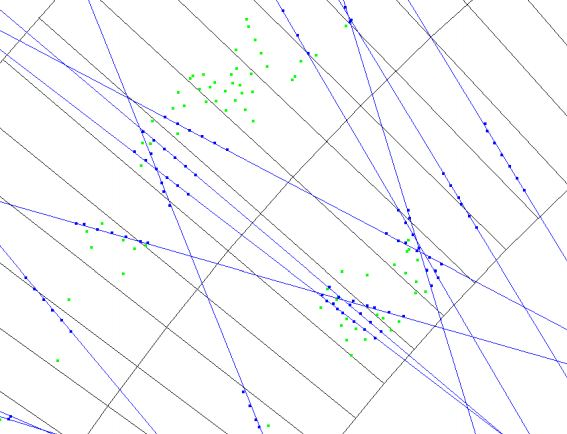
\includegraphics[width=0.7\textwidth]{Figures/houghtransformcartoon.JPG}
    \rule{35em}{0.5pt}
  \caption[Hits in the DC matched to tracks using a Hough transform]{Hits in the DC matched to tracks using a Hough transform. Note that if we were to ignore the track lines it would just be a collection of points. CHT aims to provide these matched track lines by weighting combinatoric solutions by probability of it being a physical track.}
  \label{fig:houghtransform}
\end{figure}

\begin{figure}[htbp!]
  \centering
    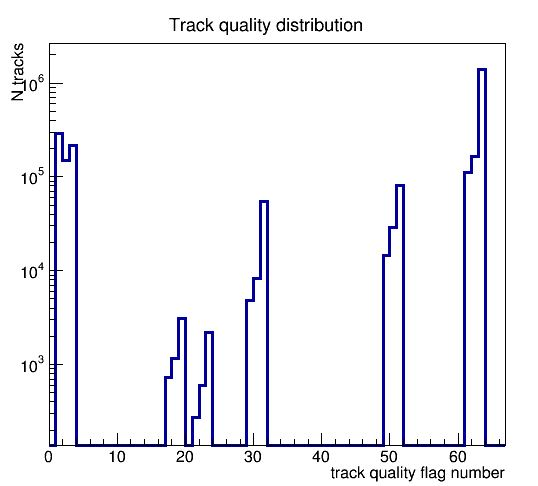
\includegraphics[width=0.5\textwidth]{evtQA/trackqualitydist.JPG}
    \rule{35em}{0.5pt}
  \caption[Distribution of track quality.]{Distribution of track quality by track quality flag designation.}
  \label{fig:trkquality}
\end{figure}

\subsubsection{Track Matching: TOF and PC3}
The magnetic field in PHENIX is strongest in the IR where $R<2$ and negilgible within the central arms\citep{rolnickthesis}. Therefore once tracks are matched in the DC and through the PC1 we can project the track linearly through the rest of the central arms. We can then match these projections with hits in the PC3 and TOF as illustrated in figure \ref{fig:pc3tofmatching} and assign variables (called \textit{residuals}) to the difference between where a hit landed in the TOF/PC3 versus where it was projected to be, one in azimuthal angle ($d\phi$) and one along beam axis ($dz$). Therefore, track purity can be increased by setting limits to how large a track's residuals can be, usually in multiples of standard deviations from a probability distribution around the projected TOF/PC3 hit. For this analysis, the maximum residual allowed for both TOF and PC3 in both $z$ and $\phi$ is three standard deviations ($3\sigma$) to allow for more statistics needed due to the lower multiplicity d+Au system (compared to larger systems) while still maintaining good track reconstruction purity.
\begin{figure}[htbp!]
  \centering
    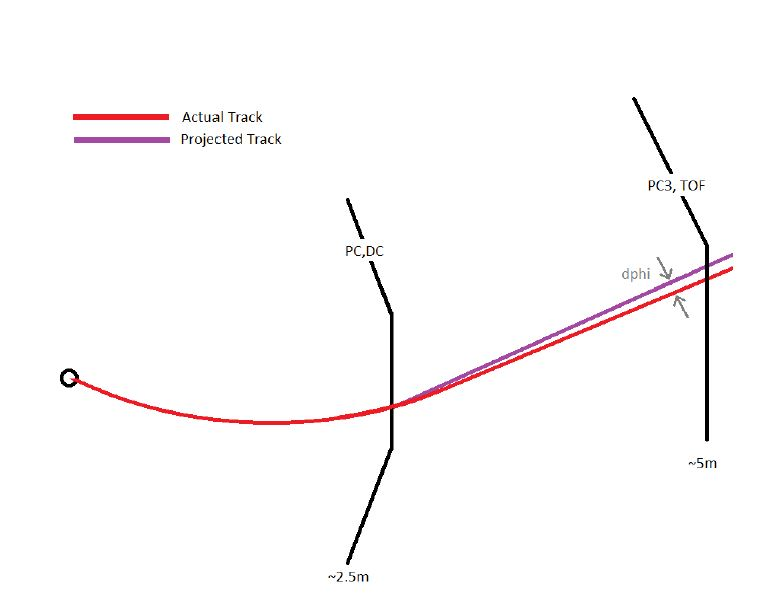
\includegraphics[width=0.9\textwidth]{Figures/pc3tofmatching.JPG}
    \rule{35em}{0.5pt}
  \caption[Diagram of track reconstruction by the DC/PC1 projected linearly onto the TOF/PC3]{Diagram of track reconstruction by the DC/PC1 projected linearly onto the TOF/PC3. \citep{schaeferthesis}}
  \label{fig:pc3tofmatching}
\end{figure}

\subsection{Particle Identification}
\label{sect:pidmethod}
Using the TOF detectors' high resolution timing measurements I am able to identify particles which have long lifetime relative to the event duration i.e. particles whose lifetimes are long enough such that they do not decay before leaving the detector. For this analysis, these particles of interest are the charged pions ($\pi^{\pm}$), charged kaons ($k^{\pm}$), and protons/antiprotons ($p/\bar{p}$). Since the masses of these particles are distinct, plotting the momentum vs time of flight can show clear separation between pion, kaon, and proton signals (see fig \ref{fig:tofchargemom}). 

\begin{figure}[htbp!]
  \centering
    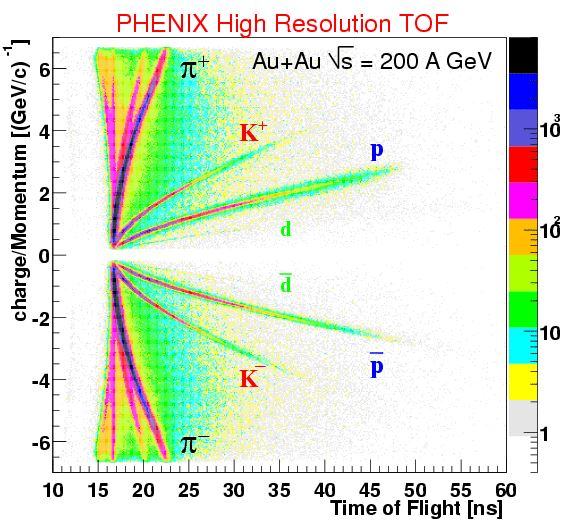
\includegraphics[width=0.7\textwidth]{Figures/tofchargemom.JPG}
    \rule{35em}{0.5pt}
  \caption[Particle separation in the TOF]{Particle separation in the TOF \citep{tofchargemom}}
  \label{fig:tofchargemom}
\end{figure}

While visually the individual particle signatures are easily identifiable in this plot, computationally it is advantageous to convert units so that the signatures only depend on a single variable. After the collision, the QGP fireball is expanding rapidly however the constituent outgoing tracks traversing the distance scales in the detector do not experience appreciable deceleration. We know from basic kinematics that we can calculate the velocity, v, of an object traveling at a constant speed:

\begin{equation}
v=\frac{L}{t} \implies t=\frac{L}{v},
\end{equation}
where t is the time it takes to travel some path length, L. It is useful to define the relative speed of the particle compared to the speed of light, c, as $\beta = v/c$ and substitute it in for v. We also know from the relativistic identities that $\beta = p/E$ and $E^{2} = p^{2} + m^{2}$. The equation is then: 

\begin{equation}
t=\frac{L}{v} = t=\frac{L}{c\beta} = \frac{L}{c} \frac{E}{p} = \frac{L}{c} \frac{\sqrt{p^{2} + m^{2}}}{p}.
\end{equation}

which can be solved for $m^{2}$ to give the mass vs time relation:

\begin{equation} \label{eqn:m2tof}
m^{2} = p^{2} \bigg\{ \frac{t^{2}}{L^{2}} -1 \bigg\}.
\end{equation}

Note that since the distance from the event vertex to the detector is constant and for that distance scale the velocity, and therefore also the momentum, can be treated as constant, $m^{2}$ depends on two constant terms if we take measurements in bins of p. Since we are talking about radially outward traveling tracks, this p is, in practice, $p_{T}$. Therefore if we do arithmetic on the track variables we are able to plot $m^{2}$ vs $p_{T}$ which gives us a much easier to analyze representation of the individual particle signatures.

\begin{figure}[htbp!]
  \centering
    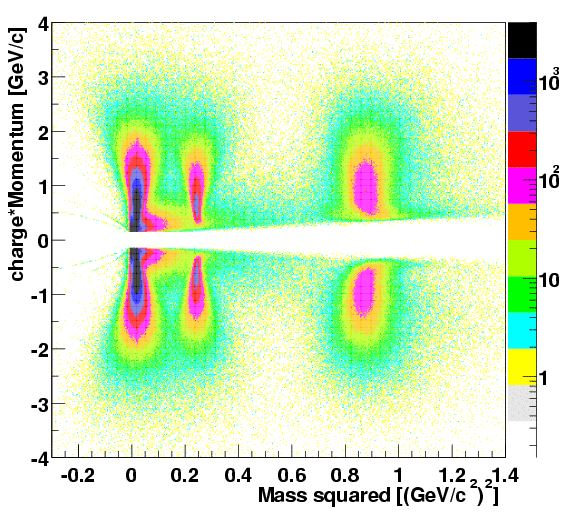
\includegraphics[width=0.7\textwidth]{Figures/m2tofvspt.jpg}
    \rule{35em}{0.5pt}
  \caption[$m^{2}$ vs $p_{T}$ showing clear constant separation of particle signatures.]{$m^{2}$ vs $p_{T}$ showing clear constant separation of particle signatures. \citep{tofchargemom}}
  \label{fig:m2tofvspt}
\end{figure}

\pagebreak
\pagebreak
